%%%%%%%% ICML 2023 EXAMPLE LATEX SUBMISSION FILE %%%%%%%%%%%%%%%%%

\documentclass{article}

% Recommended, but optional, packages for figures and better typesetting:
\usepackage{microtype}
\usepackage{graphicx}
\usepackage{subcaption}
\usepackage{booktabs} % for professional tables

\usepackage{tikz}
% Corporate Design of the University of Tübingen
% Primary Colors
\definecolor{TUred}{RGB}{165,30,55}
\definecolor{TUgold}{RGB}{180,160,105}
\definecolor{TUdark}{RGB}{50,65,75}
\definecolor{TUgray}{RGB}{175,179,183}

% Secondary Colors
\definecolor{TUdarkblue}{RGB}{65,90,140}
\definecolor{TUblue}{RGB}{0,105,170}
\definecolor{TUlightblue}{RGB}{80,170,200}
\definecolor{TUlightgreen}{RGB}{130,185,160}
\definecolor{TUgreen}{RGB}{125,165,75}
\definecolor{TUdarkgreen}{RGB}{50,110,30}
\definecolor{TUocre}{RGB}{200,80,60}
\definecolor{TUviolet}{RGB}{175,110,150}
\definecolor{TUmauve}{RGB}{180,160,150}
\definecolor{TUbeige}{RGB}{215,180,105}
\definecolor{TUorange}{RGB}{210,150,0}
\definecolor{TUbrown}{RGB}{145,105,70}

% hyperref makes hyperlinks in the resulting PDF.
% If your build breaks (sometimes temporarily if a hyperlink spans a page)
% please comment out the following usepackage line and replace
% \usepackage{icml2023} with \usepackage[nohyperref]{icml2023} above.
\usepackage{hyperref}


% Attempt to make hyperref and algorithmic work together better:
\newcommand{\theHalgorithm}{\arabic{algorithm}}

\usepackage[accepted]{icml2023}

% For theorems and such
\usepackage{amsmath}
\usepackage{amssymb}
\usepackage{mathtools}
\usepackage{amsthm}

% if you use cleveref..
\usepackage[capitalize,noabbrev]{cleveref}

%%%%%%%%%%%%%%%%%%%%%%%%%%%%%%%%
% THEOREMS
%%%%%%%%%%%%%%%%%%%%%%%%%%%%%%%%
\theoremstyle{plain}
\newtheorem{theorem}{Theorem}[section]
\newtheorem{proposition}[theorem]{Proposition}
\newtheorem{lemma}[theorem]{Lemma}
\newtheorem{corollary}[theorem]{Corollary}
\theoremstyle{definition}
\newtheorem{definition}[theorem]{Definition}
\newtheorem{assumption}[theorem]{Assumption}
\theoremstyle{remark}
\newtheorem{remark}[theorem]{Remark}

% Todonotes is useful during development; simply uncomment the next line
%    and comment out the line below the next line to turn off comments
%\usepackage[disable,textsize=tiny]{todonotes}
\usepackage[textsize=tiny]{todonotes}


% The \icmltitle you define below is probably too long as a header.
% Therefore, a short form for the running title is supplied here:
\icmltitlerunning{Project Report Template for Data Literacy 2023/24}

\begin{document}

\twocolumn[
\icmltitle{A Data-Driven Perspective on Human Error as a Cause of Fatal Traffic Accidents}


% It is OKAY to include author information, even for blind
% submissions: the style file will automatically remove it for you
% unless you've provided the [accepted] option to the icml2023
% package.

% List of affiliations: The first argument should be a (short)
% identifier you will use later to specify author affiliations
% Academic affiliations should list Department, University, City, Region, Country
% Industry affiliations should list Company, City, Region, Country

% You can specify symbols, otherwise they are numbered in order.
% Ideally, you should not use this facility. Affiliations will be numbered
% in order of appearance and this is the preferred way.
\icmlsetsymbol{equal}{*}

\begin{icmlauthorlist}
\icmlauthor{Leon Trochelmann}{equal,first}
\icmlauthor{Jonathan Ranck}{equal,second}
\icmlauthor{Paul-Henrik Heilmann}{equal,third}
\icmlauthor{Filippo Albani}{equal,fourth}
\end{icmlauthorlist}

% fill in your matrikelnummer, email address, degree, for each group member
\icmlaffiliation{first}{Matrikelnummer 6646000, leon.trochelmann@student.uni-tuebingen.de, MSc Machine Learning}
\icmlaffiliation{second}{Matrikelnummer 6230070, jonathan.ranck@student.uni-tuebingen.de, BSc Physics}
\icmlaffiliation{third}{Matrikelnummer 16648314, paul-henrik.heilmann@student.uni-tuebingen.de, MSc Machine Learning}
\icmlaffiliation{fourth}{Matrikelnummer 6638113, filippo.albani@student.uni-tuebingen.de, MSc Physics}

% You may provide any keywords that you
% find helpful for describing your paper; these are used to populate
% the "keywords" metadata in the PDF but will not be shown in the document
\icmlkeywords{Human Error, Transportation, Analysis, Accidents}

\vskip 0.3in
]

% this must go after the closing bracket ] following \twocolumn[ ...

% This command actually creates the footnote in the first column
% listing the affiliations and the copyright notice.
% The command takes one argument, which is text to display at the start of the footnote.
% The \icmlEqualContribution command is standard text for equal contribution.
% Remove it (just {}) if you do not need this facility.

%\printAffiliationsAndNotice{}  % leave blank if no need to mention equal contribution
\printAffiliationsAndNotice{\icmlEqualContribution} % otherwise use the standard text.


\begin{abstract}
%% Put your abstract here. Abstracts typically start with a sentence motivating why the subject is interesting. Then mention the data, methodology or methods you are working with, and describe results. 
%X is a widely used technique, but can’t do Y. We show that X can actually be interpreted as Z, thus the wonderful technique known as $Z_Y$ can be applied to X to do Y. This means that X can now also be applied/scaled/extended to do various cool things. We demonstrate this in several experiments on real-world data from the domain of D.

Human error in motor vehicle driving, historically distinguished from mechanical errors, faces evolving considerations, particularly in the era of automated vehicles. This study introduces a new data-driven definition of human error using the FARS2021National dataset of fatal U.S. traffic accidents. Our analysis reveals a high occurrence of human error within these accidents, also demonstrating strong correlations with driver demographics and the time of day. The high incidence of preventable risk factors in fatal accidents underscores the need for new solutions to enhance road safety in the United States.

\end{abstract}


\section{Introduction}\label{sec:intro}

%% Motivate the problem, situation or topic you decided to work on. Describe why it matters (is it of societal, economic, scientific value?). Outline the rest of the paper (use references, e.g.~to \Cref{sec:methods}: What kind of data you are working with, how you analyse it, and what kind of conclusion you reached. The point of the introduction is to make the reader want to read the rest of the paper.

%TODO: Specify which correlations we observe.

Human error is a contested term with several accepted definitions \citep{reason2000human, woods2017behind, strauch2017investigating}. In the context of motor vehicle driving it has traditionally been used to differentiate from mechanical error \citep{stanton2009human}, but for example, in the modern context of automated motor vehicles, we may also be interested in considering errors that are specific to human drivers.
\\
In this work, we introduce a new data-driven definition of such human error, allowing us to differentiate these human errors from those that may be consequences of the distinct challenges of the driving scenario \citep{guanetti2018control}. We base our definition on the FARS2021National dataset \citep{fars} of fatal traffic accidents in the United States of America and analyse the occurrence of human error within it. 
\\
Our results show an overall high occurrence of cases involving human errors in the United States. We also observe a strong correlation of human error occurrence with the demographics of the involved drivers and the time of day of the accident.
\\
Ultimately, these results reflect a significant number of possibly preventable traffic fatalities, presenting evidence of the shortcomings of human drivers that motivate improvements of road traffic safety in the United States.

% Section Introduction:
% - (status quo) Mention that self-driving cars are often motivated by an assumption that car accidents are avoidable and caused by "human error"
% - (problem with the status quo) However, human error is never clearly defined and claims that "90% of car accidents are caused by human error" have no basis to substantiate them
% - (proposed improvment) This is where our project comes in, offering a way to quantify certain preventable human error of which we can be sure that it would not be made by automated cars
% - Outline the paper
%     - Mention which data was used and to what end
%     - Mention which methods were used and to what end
% - Very briefly summarise the takeaways from the results and their implication (contributions)

% From lecture notes:
% - Motivate the idea and the contributions
% - Would be good to have a lot of citations to undermine importance 
%	(note: scholar has a few papers on human error in general, 
%	there's a paper on the difficulties of making a good human error model,
% 	and one about motorcycles)
% - Promise, don't explain

% There is one key paper to reference: "Human error taxonomies applied to driving" on scholar
% - 15 years old, and analysis of error frequency based on data that is almost 50 years old
% - attempts very complex
% - might be able to connect this to the paper on the difficulties of making a useful error model

\section{Data and Methods}\label{sec:methods}

%% In this section, describe \emph{what you did}. Roughly speaking, explain what data you worked with, how or from where it was collected, it's structure and size. Explain your analysis, and any specific choices you made in it. Depending on the nature of your project, you may focus more or less on certain aspects. If you collected data yourself, explain the collection process in detail. If you downloaded data from the net, show an exploratory analysis that builds intuition for the data, and shows that you know the data well. If you are doing a custom analysis, explain how it works and why it is the right choice. If you are using a standard tool, it may still help to briefly outline it. Cite relevant works. You can use the \verb|\citep| and \verb|\citet| commands for this purpose \citep{mackay2003information}.

%% This is the template for a figure from the original ICML submission pack. In lecture 10 we will discuss plotting in detail.
%% Refer to this lecture on how to include figures in this text.
%% 
%% \begin{figure}[ht]
%% \vskip 0.2in
%% \begin{center}
%% \centerline{\includegraphics[width=\columnwidth]{icml_numpapers}}
%% \caption{Historical locations and number of accepted papers for International
%% Machine Learning Conferences (ICML 1993 -- ICML 2008) and International
%% Workshops on Machine Learning (ML 1988 -- ML 1992). At the time this figure was
%% produced, the number of accepted papers for ICML 2008 was unknown and instead
%% estimated.}
%% \label{icml-historical}
%% \end{center}
%% \vskip -0.2in
%% \end{figure}

% Section Data and Methods:
% 	- Outline the section and mention the core idea of our approach
% 	Subsection Data:
%		- Introduce the data properly and in more detail (replacement for missing background section)
%		- Elaborate on aspects of the data relevant to us and tell why they're relevant
% 	Subsection Human Error:
%		- Describe our definition of human error in detail
%	Subsection Analysis:
%		- Describe our analysis on the role of human error as analysis of conditional probabilities
%		- Mention the two phases of our analysis in terms of first finding large human error correlation, and then further analysing which specific errors contribute to the high correlation
%		- Describe the actual experiments  one by one

We introduce the dataset we considered for our analysis and show how it leads to our definition of human error. This definition is motivated by a number of factors which we explain in detail, followed by a description of our analysis.

% TODO:
% - Specify total amount of cases to emphases why it presents a rich body for the analysis
% - add reference for contents/documentation of the fars dataset?
% - add number for total car accidents
% - add example for fars contents
% - add example for variable with no correlation
% - generally add more examples and some minimal figures or tables
% - ascertain whether specifics of variable selection should be documented


% Cite google data as information about county populations with https://github.com/google-research/open-covid-19-data


\subsection{Dataset}
Out of the many possible choices for a dataset on car accidents, we decided to use the FARS2021National dataset by the United States of America's National Highway Traffic Safety Administration. The FARS (Fatality Analysis Reporting System) aims to register all fatal car accidents that occur in the USA in any given year.
\\
FARS captures a large amount of information about each accident, including information about all persons and vehicles involved in the accident, as well as the circumstances of the accident itself. Figure \ref{fig:fars-cases} illustrates the raw distribution of recorded cases in the United States in the year 2021. This presents a rich body of information upon which we base our analysis !why?!.
\begin{figure}[ht]
	\vskip 0.2in
	\begin{center}
		\includegraphics[width = \columnwidth]{plots/fars-cases}
		\caption{Cases of road traffic fatalities in the United States of America in the year 2021 grouped by state.}
		\label{fig:fars-cases}
	\end{center}
	\vskip -0.2in
\end{figure}
\\
Zoning in on fatal car accidents explicitly is a useful abstraction, as it reduces ambiguity over the crash severity !specify!. Additionally, the number of estimated total car accidents is not only very high !source!, but accidents are also often not reported or investigated in sufficient detail !source!.



\subsection{Defining Human Error}
To analyse human error, we define it based on a selection of variables that we consider to be both reflect error and arise from the human condition specifically. This selection notably excludes risk factors that may not be preventable, such as disabilities. It furthermore disregards risk factors that do not arise from the human condition, such as the weather.\\
Finally, we choose a conservative approach of only selecting risk factors which are generally known to cause many traffic accidents. While these risk factors are not guaranteed to be the true underlying cause of the accident, they can generally be accepted as likely causes.
\\
Specific to FARS2021National we choose the variables speeding, driving without a valid license and driving under the influence to constitute human error. Figure \ref{fig:err-case-counts} illustrates the respective variables, their number of occurrences and their overlap.

\begin{figure}[ht]
	\vskip 0.2in
	\begin{center}
		\centerline{\includegraphics[width=0.66\columnwidth]{placeholder}}
		\caption{Case counts for the three variables we consider as human error in FARS2021National.}
		\label{fig:err-case-counts}
	\end{center}
	\vskip -0.2in
\end{figure}

First, we consider a case to have speeding if the driver went over the speed limit. Second, we consider it to be driving without a license if the driver did not have a valid license. Third, we consider driving under the influence, subject to the judgement of law enforcement. Finally, we introduce human error as a new variable that is TRUE if one of these indicators is given and FALSE otherwise. We will consider only this definition of human error in our analysis.
\\
FARS2021National includes several cases !whats the number?! where the value of some of these variables is missing. We have excluded these cases from the dataset for our analysis.

\section{Experiments and Results}\label{sec:results}

%% In this section outline your results. At this point, you are just stating the outcome of your analysis. You can highlight important aspects (``we observe a significantly higher value of $x$ over $y$''), but leave interpretation and opinion to the next section. This section absoultely \emph{has} to include at least two figures.

To demonstrate the significance of human error and show how it interacts with other variables, we analyse the occurrence rates of human error. First, we analyse the general occurrence of human error in our dataset. Second, we investigate how human error is correlated with other variables.
\\
The FARS datasets contain a wide range of variables, many of which have no significant correlation with human error. We present several significant correlations our analysis yielded, but we do not claim completeness. A full correlation analysis with every variable in the FARS is beyond the scope of this work.

\subsection{Occurence}
Figure \ref{fig:occurence} shows that the human error under our consideration is a common occurrence in the dataset. This statistic in and of itself urges \ldots

\begin{figure}[ht]
	\vskip 0.2in
	\centering
		\begin{subfigure}[ht]{0.45\columnwidth}
			\includegraphics[width=\columnwidth]{placeholder}
			\caption{The prevalence of the variables and their values we consider human error as a percentage of all cases.}
			\label{prevalence-per-variable}
		\end{subfigure}
		\hfill
		\begin{subfigure}[ht]{0.45\columnwidth}
			\includegraphics[width=\columnwidth]{placeholder}
			\caption{Number of human error cases attributed to each variable.}
			\label{prevalence-multiple-occurence}
		\end{subfigure}
	\caption{\ldots}
	\label{fig:occurence}
	\vskip 0.2in
\end{figure}

\subsection{Correlations}
The variables most strongly correlated with human error are those on the driver and the conditions of the accident.
\\
We analyse the demographics of human error by conditioning on age and sex. The results are illustrated in figure \ref{fig:err-demography}. Trivially, the human error rate is 1 for all age groups below the minimum legal driving age in the USA. One can also that the incidence of human error is overall higher in the male population.\\
Additionally, older age groups have less human error incidence. The peaks for human error incidence vary between the male and female populations, with the male population having a peak in the ? to ? age group, and the female population has a peak in the ? to ? age group.\\

\begin{figure}[ht]
	\vskip 0.2in
	\begin{center}
		\centerline{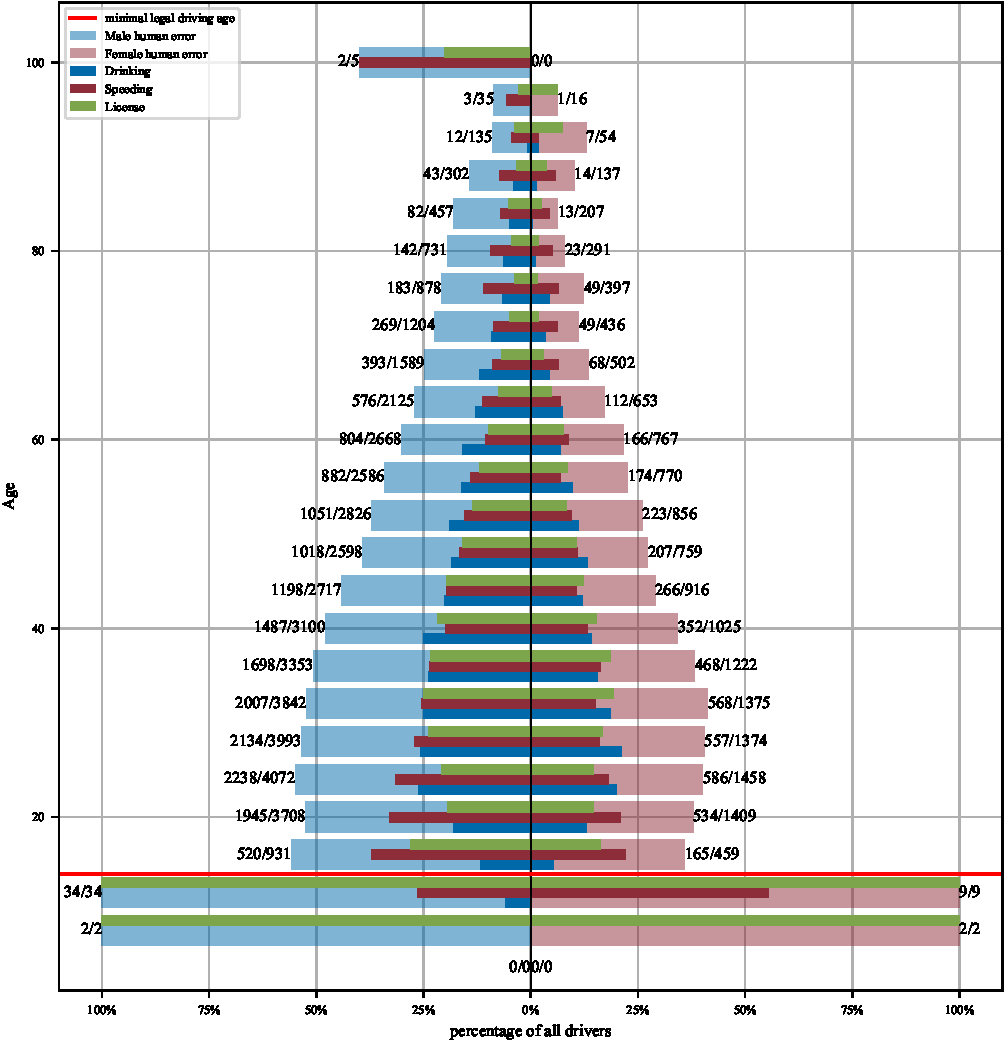
\includegraphics[width=\columnwidth]{plots/err-demography}}
		\caption{Correlation of human error with age and sex as a percentage of cases. The male population is displayed on the left and the female population on the right. The minimal legal driving age of !? source, reference ?! is located right inbetween ? the second and third ? bins.}
		\label{fig:err-demography}
	\end{center}
	\vskip -0.2in
\end{figure}

The time of day also has a significant correlation with human error, as figure \ref{fig:err-time} shows. There is a noticeable increase in all aspects of human error towards the later hours of the day and during the early night. In the case of drunk driving in particular, their distribution is heavily concentrated between the hours of 15:00 to 04:00.

\begin{figure}[ht]
	\vskip 0.2in
	\centering
		\begin{subfigure}[ht]{0.45\columnwidth}
			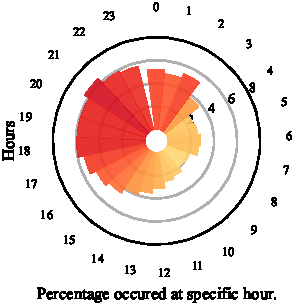
\includegraphics[width=\columnwidth]{plots/err-time-total}
			\caption{Incidence of human error by hour of day.}
			\label{fig:err-time-overall}
		\end{subfigure}
		\hfill
		\begin{subfigure}[ht]{0.45\columnwidth}
			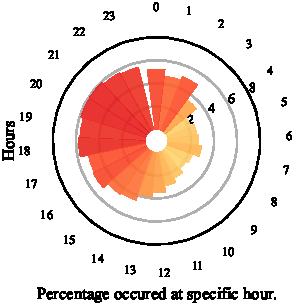
\includegraphics[width=\columnwidth]{plots/err-time-speeding}
			\caption{Incidence of speeding by hour of day.}
			\label{fig:err-time-speeding}
		\end{subfigure}

		\vskip\baselineskip
		\begin{subfigure}[ht]{0.45\columnwidth}
			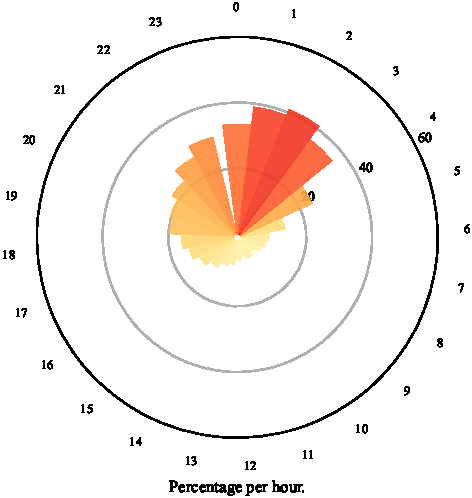
\includegraphics[width=\columnwidth]{plots/err-time-drinking}
			\caption{Incidence of drunk driving by hour of day.}
			\label{prevalence-multiple-occurence}
			\label{fig:err-time-drinking}
		\end{subfigure}
		\hfill
		\begin{subfigure}[ht]{0.45\columnwidth}
			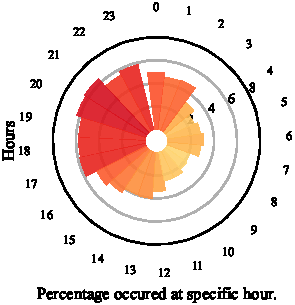
\includegraphics[width=\columnwidth]{plots/err-time-license}
			\caption{Incidence of unlicensed driving by hour of day.}
			\label{fig:err-time-license}
		\end{subfigure}
		\vskip\baselineskip
		\begin{subfigure}[ht]{\columnwidth}
			\includegraphics[width=\columnwidth]{plots/err-time-bar}
			\caption{Colour bar?}
			\label{fig:err-time-bar}
		\end{subfigure}
	\caption{The correlation of time of day in hours with human error as a \ldots}
	\label{fig:err-time}
	\vskip 0.2in
\end{figure}

A closer look at how time correlates with occurrence of human error ? plot ?


\section{Discussion \& Conclusion}\label{sec:conclusion}

%% Use this section to briefly summarize the entire text. Highlight limitations and problems, but also make clear statements where they are possible and supported by the analysis. 

In this work, we have introduced a data-driven definition of human error and demonstrated its high occurrence based on a vast dataset of fatal car accidents.
\\
Our results show that preventable risk factors have a significant incidence of fatal accidents. They also show that the incidence is correlated with the demography of drivers and the time of day ? and weekday?.
\\
Due to our conservative approach to variable selection, these rates of occurrence can also be seen as lower bounds on the true rate of preventable human error, as we did not consider difficult-to-assess factors like road rage and reckless driving.
\\
Our analysis is based on traffic data that stems exclusively from the USA in the year 2021. Other countries might experience other rates of occurrence and they may change over time.
\\
Overall, the presence of significant quantities of preventable human error motivates changes in the motorway traffic system in the USA, whether these solutions be automotive, legislative or societal. 


\section*{Contribution Statement}

%% Explain here, in one sentence per person, what each group member contributed. For example, you could write: Max Mustermann collected and prepared data. Gabi Musterfrau and John Doe performed the data analysis. Jane Doe produced visualizations. All authors will jointly wrote the text of the report. Note that you, as a group, a collectively responsible for the report. Your contributions should be roughly equal in amount and difficulty.
Etiam aliquet hendrerit lectus porttitor placerat. Nulla ac nisl enim. Nunc vulputate augue vitae erat hendrerit tempus. Proin dolor nulla, accumsan at risus ac, volutpat bibendum nulla. Donec porttitor varius facilisis. Praesent at urna nulla. Duis eleifend nulla id quam auctor mollis. Nulla facilisi.\\
\\


% \section*{Notes} 

% Your entire report has a \textbf{hard page limit of 4 pages} excluding references. (I.e. any pages beyond page 4 must only contain references). Appendices are \emph{not} possible. But you can put additional material, like interactive visualizations or videos, on a githunb repo (use \href{https://github.com/pnkraemer/tueplots}{links} in your pdf to refer to them). Each report has to contain \textbf{at least three plots or visualizations}, and \textbf{cite at least two references}. More details about how to prepare the report, inclucing how to produce plots, cite correctly, and how to ideally structure your github repo, will be discussed in the lecture, where a rubric for the evaluation will also be provided.

\bibliography{bibliography}
\bibliographystyle{icml2023}

\end{document}


% This document was modified from the file originally made available by
% Pat Langley and Andrea Danyluk for ICML-2K. This version was created
% by Iain Murray in 2018, and modified by Alexandre Bouchard in
% 2019 and 2021 and by Csaba Szepesvari, Gang Niu and Sivan Sabato in 2022.
% Modified again in 2023 by Sivan Sabato and Jonathan Scarlett.
% Previous contributors include Dan Roy, Lise Getoor and Tobias
% Scheffer, which was slightly modified from the 2010 version by
% Thorsten Joachims & Johannes Fuernkranz, slightly modified from the
% 2009 version by Kiri Wagstaff and Sam Roweis's 2008 version, which is
% slightly modified from Prasad Tadepalli's 2007 version which is a
% lightly changed version of the previous year's version by Andrew
% Moore, which was in turn edited from those of Kristian Kersting and
% Codrina Lauth. Alex Smola contributed to the algorithmic style files.
